\documentclass{beamer}
\usepackage{beamerthemesplit} % new 
\usepackage{mathrsfs}
\usepackage[normalem]{ulem}

\usetheme{default}
%\useoutertheme{infolines}
%\setbeamertemplate{navigation symbols}{gd} 

\begin{document}


\title{The Scalable Commutativity Rule: \\
Designing Scalable Software for Multicore Processors} 
\author{Presented by Jinliang Wei} 
\date{\today} 

\frame{\titlepage} 

%\frame{\frametitle{Table of contents}\tableofcontents} 

\begin{frame}
\frametitle{What's this paper about?}

\begin{itemize}
\item The authors claim that scalability is not only an implementation property 
but also an interface property.
\item Current approach to scalable software development is workload-driven.
\begin{itemize}
\item Design $\rightarrow$ implement $\rightarrow$ measure $\rightarrow$ repeat.
\item New workload? new architecture?
\item Bottleneck may be in the interface.
\end{itemize}
\item The scalable commutativity rule (informally): \\
``whenever interface operations commute, they can be implemented in a way that scales".
\end{itemize}

\end{frame}

\begin{frame}
  \frametitle{Intuition first}
Operations commute \\
 $\Rightarrow$ results independent of order \\
 $\Rightarrow$ communication is unnecessary \\
 $\Rightarrow$ without communication, no conflicts \\
\footnotetext[1]{Borrowed from Clements' SOSP 2013 presentation}
\end{frame}

\begin{frame}
\frametitle{Conflicts imply poor scalability}
Conflict: one processor writes a cache line that other processors write or
 read.
 
 \begin{figure}
   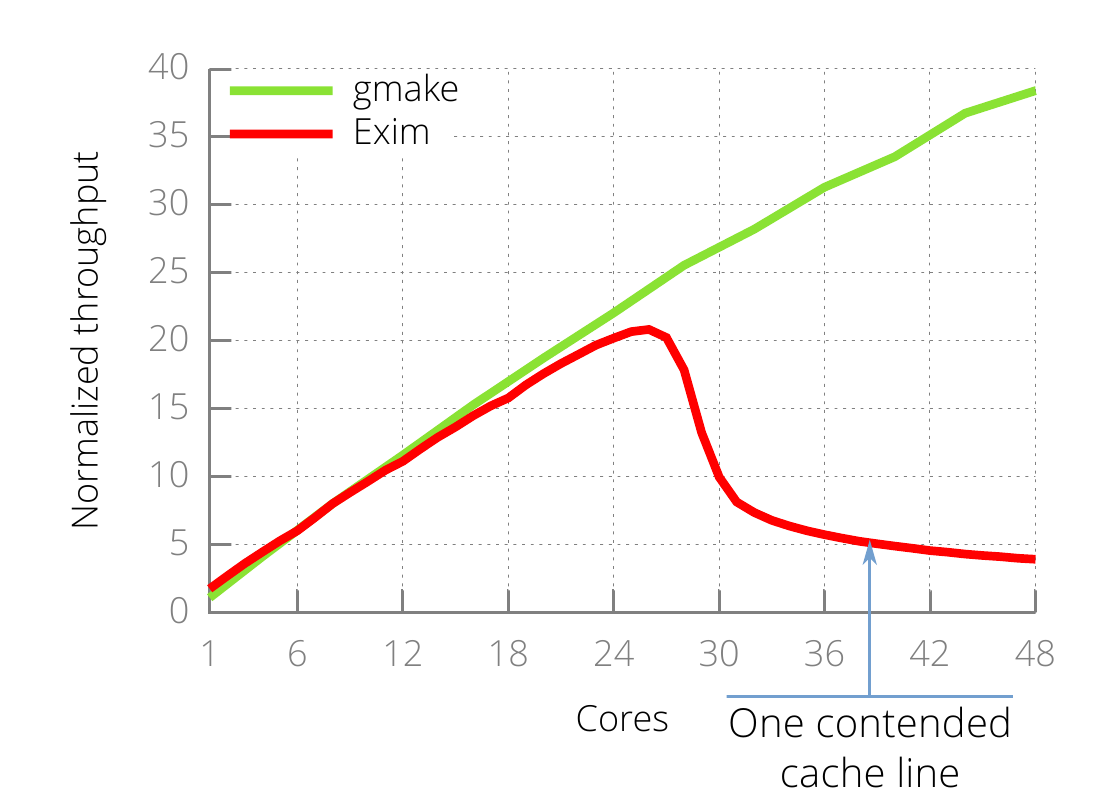
\includegraphics[width=0.8\textwidth]{799-s14-docs/cache_line_contention.png}
 \end{figure}

\footnotetext[1]{Figure borrowed from Clements' SOSP 2013 presentation}
\end{frame}

\begin{frame}
\frametitle{The scalability rule}
Assume a \uline{specification} $\mathscr{S}$ with a correct reference 
implementation M. Consider a \uline{history} $H = X || Y$ where $Y$ 
\uline{SIM-commutes} in $H$, 
and where M can generate $H$. Then there exists a correct implementation m of 
$\mathscr{S}$ whose steps in the $Y$ region of $H$ are conflict-free.
\end{frame}

\begin{frame}
\frametitle{Some teminology}

\begin{itemize}
\item A system execution is a sequence of \emph{action}s.
\begin{itemize}
\item An \emph{action}: either an \emph{invocation} or a \emph{response}.
\end{itemize}
\item A system execution is called a \emph{history}.
\begin{itemize}
\item \emph{Well-formed}: each thread's invocations and responses are in pairs.
\end{itemize}
\item The \emph{specification} distinguishes whether or not a history is 
  ``correct".
\item Reordering preserves the order of actions within each thread.
\begin{itemize}
\item $H|t = H'|t$ for every thread $t$.
\end{itemize}
\end{itemize}
\end{frame}


\begin{frame}
\frametitle{SIM-commutativity}

\begin{itemize}
\item $Y$ SI-commutes in $X||Y$ $:=$ \\
  $\forall Y' \in reorderings(Y), Z: X||Y||Z \in \mathscr{S} 
  \Longleftrightarrow X||Y'||Z \in \mathscr{S} $

\begin{itemize}
\item SI-commutativity considers reordering within a context prepared by 
previous operations (X) - state depedency.
\end{itemize}

\item $Y$ SIM-commutes in $X||Y$ $:=$ \\
  $\forall P \in prefixs(reorderings(Y)):$ P SI-commutes in $X||P$
\begin{itemize}
\item Monotonicity is needed to prove the theory.
\end{itemize}
\end{itemize}

\end{frame}

\begin{frame}
\frametitle{SIM commutativity is state-dependent}

\begin{itemize}
\item It captures operations that commute in some states but not others.
\begin{itemize}
\item Few system calls unconditionally commute.
\end{itemize}

\item An example: two calls to \texttt{open("a", O\_CREATE | O\_EXCL)}
  \begin{itemize}
    \item Often don't commute.
    \item Commute if:
      \begin{itemize}
        \item different working directory;
        \item or if the file already exists. 
        \end{itemize}
\end{itemize}
\end{itemize}
\end{frame}


\begin{frame}
  \frametitle{SIM commutativitiy is interface-based}
  \begin{itemize}
    \item It requires the reordering to be 
  \end{itemize}
\end{frame}

\end{document}

